%law_inductive
%\begin{figure}
%\centering
%\begin{minipage}[t]{0.4\textwidth}
%\centring
%\includegraohics[width=0.35\textwidth]{bilder/FIT_max_integral1}
%\caption{Integration on the edge of one single elemental plane.}
%\label{fig:FIT_max_integral1}
%\end{minipage}
%\begin{minipage}[t]{0.4\textwidth}
%\centring
%\includegraohics[width=0.35\textwidth]{bilder/FIT_max_integral2}
%\caption{Integration on the edge of one single elemental cell.}
%\label{fig:FIT_max_integral2}
%\end{minipage}
%\end{figure}


\begin{figure}
\centering
\subfigure[Integration on the edge of one single elemental plane $A_{u}(n)$]{
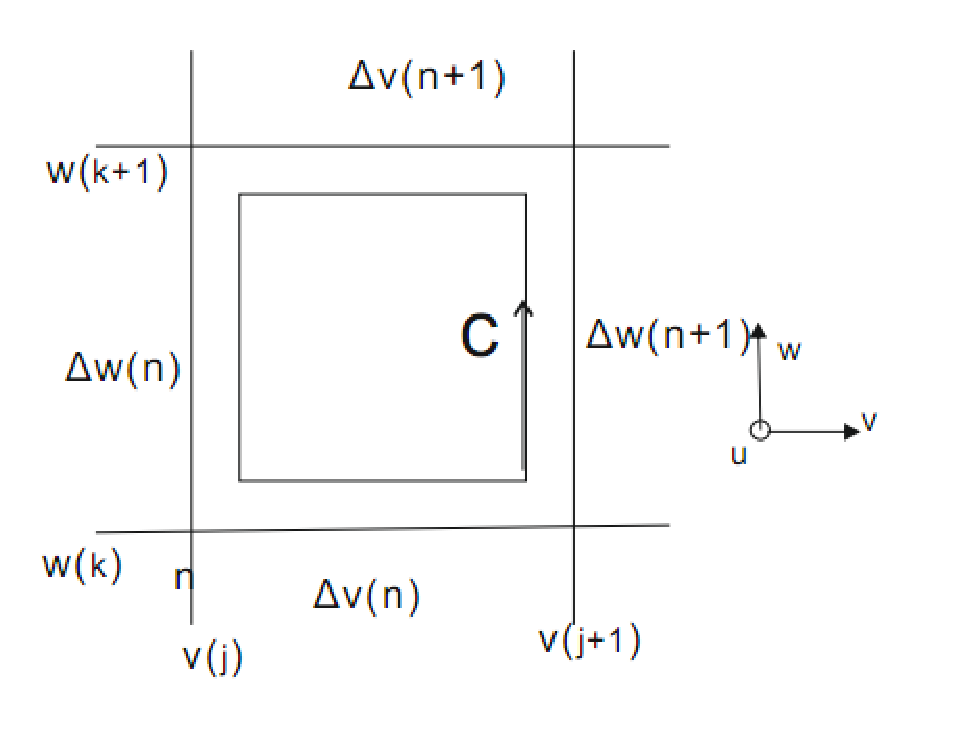
\includegraphics[width=0.35\textwidth]{bilder/FIT_max_integral1}
\label{fig:FIT_max_integral1}
}
\hfill
\subfigure[Integration on the edge of one single elemental cell]{
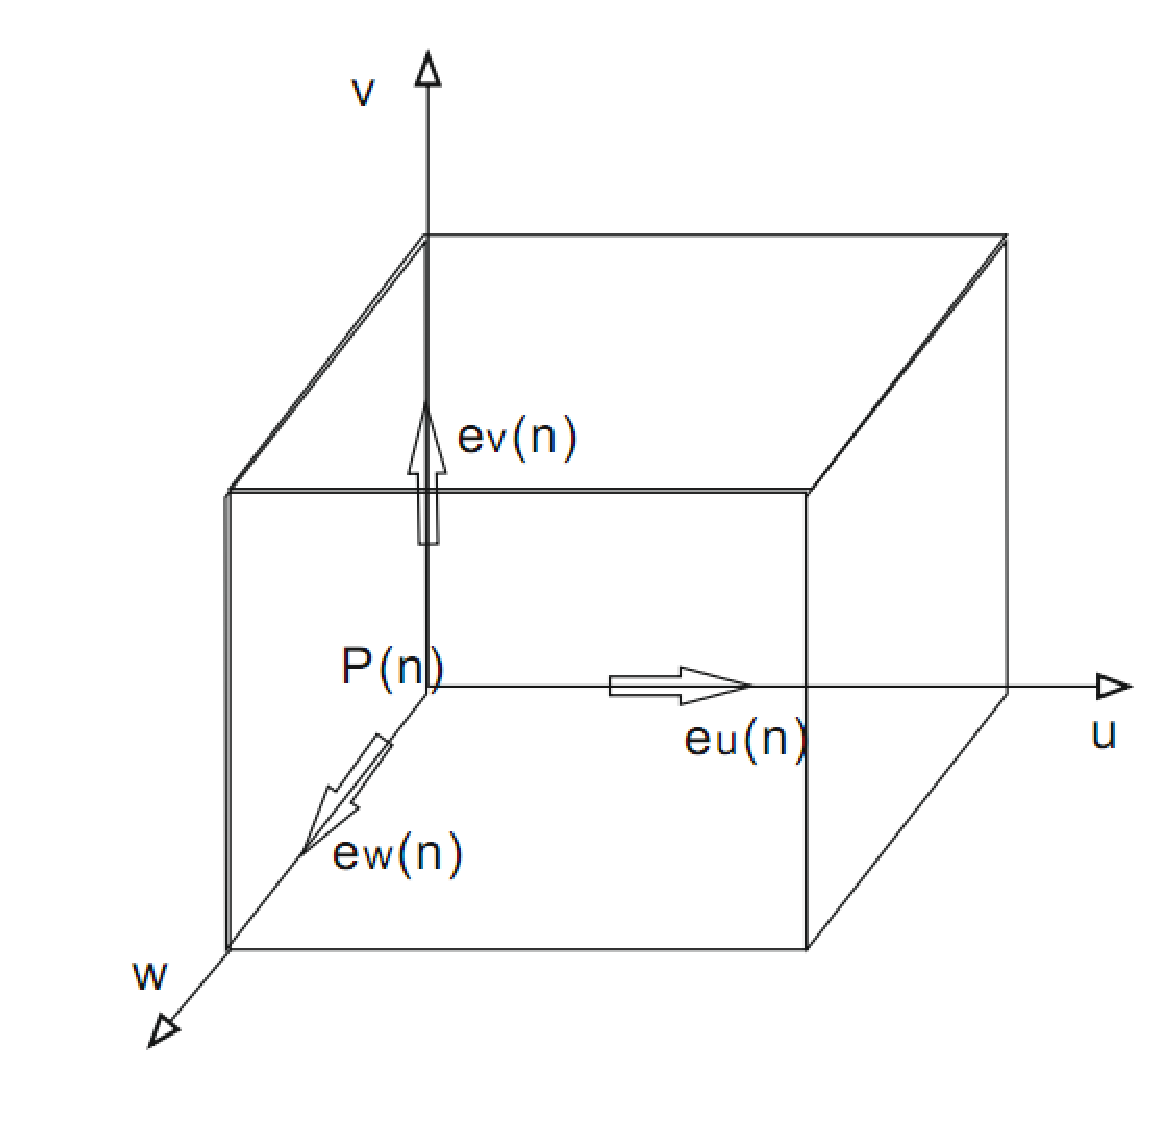
\includegraphics[width=0.35\textwidth]{bilder/FIT_max_integral2}
\label{fig:FIT_max_integral2}
}
\caption{discrete Maxwell's Equations}
\end{figure}

Followling is a demonstration of the discretized form from the  inductive law(\ref{eq:maxwell_1}). Considering the path integral in a single element edge like Fig.\ref{fig:FIT_max_integral1},the left side of (\ref{eq:maxwell_1}) can be presented as (\ref{eq:inductive_left}). 

\begin{equation}
\int_{C}\vec{E}\cdot d\vec{s}
=\underbrace{\int_{\Delta v(n)}\vec{E}\cdot d\vec{s}}_{\widehat{e_{v}(n)}}
+\underbrace{\int_{\Delta w(n+M_{v})}\vec{E}\cdot d\vec{s}}_{\widehat{e_{w}(n+M_{v})}}
-\underbrace{\int_{\Delta v(n+M_{w})}\vec{E}\cdot d\vec{s}}_{\widehat{e_{v}(n+M_{w})}}
-\underbrace{\int_{\Delta w(n)}\vec{E}\cdot d\vec{s}}_{\widehat{e_{w}(n)}}
\label{eq:inductive_left}
\end{equation}
where \widehat{e} is so called  electric grid voltage

In the mean time the right side of (\ref{eq:maxwell_1}) is transformed as (\ref{eq:inductive_right})
\begin{equation}
-\iint_A_{u}(n)\frac{\partial\vec{B}}{\partial t}\cdot\mathrm{d}\vec{A} 
=-\iint_A_{u}(n)\frac{\partial B^{*}_{u}}{\partial t}\cdot\mathrm{d}A
\approx -\frac{\partial}{\partial t}b_{u}(n)A_{u}(h)
\label{eq:inductive_right}
\end{equation}

Here $A_{u}(n)=\Delta v(n)\Delta w(n)$ and $b_{u}(n)$ is magnetic fluxe density
Define magnetic grid fluxe(\ref{eq:mag_fluxe})
\begin{equation}
\widehat{\widehat{b_{u}(n)}}=\iint_A_{u}(n)\vec{B}\cdot\mathrm{d}\vec{A}
\label{eq:mag_fluxe}
\end{equation}

surface integral